% This file is isea.tex. It contains the formatting instructions for and acts as a template for submissions to ISEA 2025. It is based on the ICCC formats and instructions. It uses the files isea.sty, isea.bst and isea.bib, the first two of which also borrow from AAAI IJCAI formats and instructions.
% Modified from ICCC.tex by B. Bogart

\documentclass[letterpaper]{article}
\usepackage{isea}
\usepackage[pdftex]{graphicx}
\usepackage{times}
\usepackage{helvet}
\usepackage{courier}
\usepackage[numbers]{natbib}
\pdfinfo{
/Title (Towards an Effective Theory of Art)
/Author (Kynan Stewart Hughes)}
% The file isea.sty is the style file for ISEA 2025 proceedings.
%
\title{Towards an Effective Theory of Art}
\author{Kynan Stewart Hughes\\
Creativity and Cognition Studios\\
University of Technology Sydney\\
Sydney, Australia\\
kynan.s.hughes@student.uts.edu.au\\
\newline
\newline
}
\setcounter{secnumdepth}{0}

\begin{document} 
\maketitle
\begin{abstract}
The Proceedings of the International Symposium on Electronic
Art will be compiled from electronic manuscripts submitted by
the authors. This paper provides brief style instructions that will
facilitate high-quality, consistent, proceedings. The title
``Abstract'' should be 10 point, bold type, centered at the
beginning of the left column. The body of the abstract
summarizing the thesis and conclusion of the paper in no more
than 200 words should be 9 point, justified, regular type.
\end{abstract}

\keywords{Keywords}

Art, technology, complexity.

\section{Introduction}

We artists, especially we artists who work with emerging technologies, are often required to explain our work, and this is a difficult task because an effective theory of art — a theory which has something useful to say about what art is and what it does or can do — has been elusive. This paper outlines an effective theory for art based on the complexity science and process philosophy. This theory may be coherently applied to any style of artistic practice It does so in a way that is accessible for artists and whichIt is especially useful for artists who engage with with emerging technologies because it describes the nature of the relationship between art and technology.  opens possibilities for connecting artmaking with other human cultural practices, both in theory and practice.

\section{Which ‘Art’?}

It is necessary to clarify what is meant by ‘art’ in this paper, because the term is used in different ways. I do not mean ‘art’ in the broadest, most general sense, as in ‘the art of war’, or if I were to say that my car mechanic is a real artist because of her skill and the care she shows in her work. Nor do I mean ‘art’ in the sense of ‘the arts’, as in ‘the arts and sciences’. Instead, I mean ‘art’ in the sense of ‘artworks’ or ‘art objects’. The things that artists make and of which we might say, ‘I don't know much about art, but I know what I like’ - or even (especially), ‘that is NOT art’. I mean the things that are displayed in galleries and museums, the things that are bought and sold, the things that are written about in art magazines and art history books, the things that we might have been taught about in art schools, the things that are made by artists.

My starting point is even more specifically a kind of art that is called ‘contemporary’ because of the way it seems to function at a certain edge of the present, and which is often characterised by a kind of self-consciousness about its own status as art and an active engagement with its current context. Art which engages with emerging technologies is always ‘contemporary’ in this sense, even if we might now be looking back in time at objects made in the past, such as the work of Nam June Paik. However, the theory I outline here is not limited to contemporary art, and it can be applied to any style practiced by artists.

Although this theory describes the kind of art that artists make, the other senses of ‘art’ are not irrelevant because, taken together, all three senses of ‘art’ operate as a set of coexisting, nested meanings that have real histories and which function together as interconnected aspects of the contemporary globalised, Westernised culture that we share to some extent. I might be a practitioner of a kind of contemporary artmaking, and specifically one that involves the material use of emerging technologies, but I am also practicing in the context of academic research that crosses certain boundaries between the arts and the sciences, and I might occasionally congratulate myself for being a real artist in the sense that I am skilled and careful in my work.

Although these different senses of ‘art’ are always present together now in our shared cultural context, they have histories. We can do a bit of a trick here, and zoom out from the present context and the present moment, and look at the history of art in the West, and see that the different senses of ‘art’ have been dominant at different times. The sense of ‘art’ as skill or craft was dominant in the ancient world - at least in the ancient Western world - and it was only later that the sense of ‘art’ as a kind of creative practice different from other kinds of crafting, began to emerge. The good news is that I'll be able stop using scare quotes around the word ‘art’ because there are some other available terms.

\section{Teche}

The word techne comes from the Greek word for art, skill, craft, and technique. Heidegger, in his essay ‘The Question Concerning Technology’, pointed out that techne is general term that includes the arts as well as the sciences, and that there was once no distinct idea of artmaking that was

% \subsection{Reified Generalities}

% As a useful constraint, I will respect is Manuel DeLanda's prohibition against using reified generalities. DeLanda has argued that a reified generality is a concept which is simply too abstract to be useful. The concept of ‘society’, for example, is a generality that only serves to shift focus away from the important features of specific societies, including their differences. Instead, DeLanda has argued, we should focus on specific, real entities. This is a useful constraint because, as well as keeping us focused, it also keeps us grounded in a materialist ontology, the foundation for this theory of art as it is for complexity science and process philosophy. Accordingly, whenever it isn't too cumbersome, I will tend to speak of, for example, ‘artworks’ or ‘art objects’ rather than ‘art’, and ‘technologies’ rather than ‘technology’.

\subsection{Length of Papers}

A variety of paper lengths will be accepted under different categories. Please note that submission lengths must be all inclusive (including references, biographies and acknowledgements).
\begin{itemize}
\item Full paper submissions can be 5-8 pages in the ISEA2025 template format.
\item Short paper submissions can be 2-4 pages in the ISEA2025 template format.
\item Poster and Demo (as extended abstracts) submissions can be up to 2 pages in the ISEA2025 template format.
\item Panel submissions can be 2-4 pages in the ISEA2025 template format.
\item Artist talk can be up to 2-4 pages in the ISEA2025 template format.
\item Institutional presentation submissions can be up to 2 pages in the ISEA2025 template format.
\item For artistic works, workshops please use the other appropriate templates.
\end{itemize}

\section{Style and Format}
Templates that implement these instructions can be retrieved at  {\small \tt http://isea2025.isea-international.org/}

\subsection{Layout}

Print manuscripts two columns to a page, in the manner in which these instructions are printed. The exact dimensions for pages are:
\begin{itemize}
\item left and right margins: 0.75''
\item column width: 3.31''
\item gap between columns: 0.38''
\item top margin—first page: 1.25''
\item top margin—other pages: 0.75''
\item bottom margin: 1.25''
\end{itemize}

\subsection{Format of Electronic Manuscript}

For the production of the electronic manuscript, you must use {\em Adobe's Portable Document Format} (PDF). Additionally, you must specify the American {\em letter} format (corresponding to 8-1/2'' x 11'') when formatting the paper.

\subsection{Blind Review}

All submission in the academic call will be reviewed in a double-blind manner.  Please do not include your affiliation and anonymize the text to keep your identity secret.

\subsection{Title and Author Information}

Center the title on the entire width of the page in a 16-point bold font. Below it, center the author name(s) in a 12-point bold font, and then center the address(es) in a 9-point regular font. Credit to a sponsoring agency can appear in the Acknowledgment Section described below.

\begin{figure}[h]
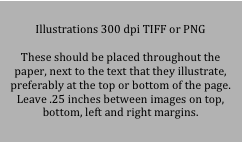
\includegraphics[width=3.31in]{figure.png}
\caption{This is an example of figure caption. Note that all figures, and tables are to be referenced in the text. \copyright Respect Copyright.}
\end{figure}

\subsection{Abstract}

The title ``Abstract'' should be 10 point, bold type, centered at the beginning of the left column. The body of the abstract summarizing the thesis and conclusion of the paper in no more than 200 words should be 9 point, justified, regular type.

\subsection{Text}

The main body of the text immediately follows the abstract. Use 10-point type in {\em Times New Roman} font.

Indent when starting a new paragraph, except after major headings. 

\subsection{Headings and Sections}

When necessary, headings should be used to separate major sections of your paper. (These instructions use many headings to demonstrate their appearance; your paper should have fewer headings.

\subsubsection{Section Headings}

Print section headings centered, in 12-point bold type in the style shown in these instructions. Your body text should be 10 point, justified, single space. Do not number sections.

\subsubsection{Subsection Headings}

Print subsection headings left justified, in 11-point bold type and mixed case (nouns, pronouns, and verbs are capitalized). They should be flush left. Your text should be 10 point, justified, single space. Do not number subsections.

\subsubsection{Subsubsection Headings}

Print subsubsection headings inline in 10-point bold type. Do not number subsubsections.

\subsubsection{Special Sections}

You may include an unnumbered acknowledgments section, including acknowledgments of help from colleagues, financial support, and permission to publish.

The references section is headed ``References,'' printed in the same style as a section heading. A sample list of references is given at the end of these instructions.  Note the various examples for books, proceedings, multiple authors, etc. 

\subsection{Footnotes}

If footnotes are necessary, place them at the bottom of the page in 9-point font. Refer to them with superscript numbers.\footnote{This is how your footnotes should appear.} Separate them from the text by a short horizontal line. 

\subsection{Quotations and Extracts}
Indent long quotations and extracts by 10 points at left margins.

\section{Acknowledgments}
The preparation of these instructions and the \LaTeX{} and Word files was facilitated by borrowing from similar documents used for ICCC proceedings.

\begin{figure*}

\includegraphics[width=\textwidth]{two-column-figure.png}
\caption{Example of a double-column figure with caption. \copyright Respect Copyright.}
\end{figure*}

\section{References}
The title “References” should be 12 point, bold style, centered. Editorial standards adhere to the guidelines set by the Chicago Manual of Style, 16th ed. References should be 9 point, regular type. List them in numerical order immediately after your essay. The numbers should be cross-referenced within the essay, with numbers placed at the end of the sentence in square brackets, with a space after the full stop, as shown at the end of this sentence. \cite{boden92}

\bibliographystyle{isea}
\bibliography{isea}

\section{Bibliography}
The title “Bibliography” should be 12 point, bold style, centered. Using 9 point, regular type, list your bibliography in alphabetical order by family name, after the references. The difference between a reference list and a bibliography is that in your references, you list all the sources you directly referred to in the body of your writing - in numerical order, whereas a bibliography includes an alphabetical listing of all those authors and sources that you have consulted while writing your essay. Use the same format as for the references otherwise.

\section{Author(s) Biography(ies)}
The title ``Author(s) Biography(ies)'' should be 12 point, bold style, centered. Using 9 point, regular type, biographies should be no longer than 150-word count.

\section{Questions?}

For technical questions about Microsoft Word formatting please seek online tutorials. For other questions about your manuscript please contact: {\tt isea2025@nabi.or.kr}


\end{document}
